\begin{figure}[!tbp]
  \centering
  % Rendered on demand from tree_approximation_ratio_3d_plot.tex.
  % Keeping the dense PGFPlots surface as a PDF avoids rebuilding it with
  % every manuscript compilation.
  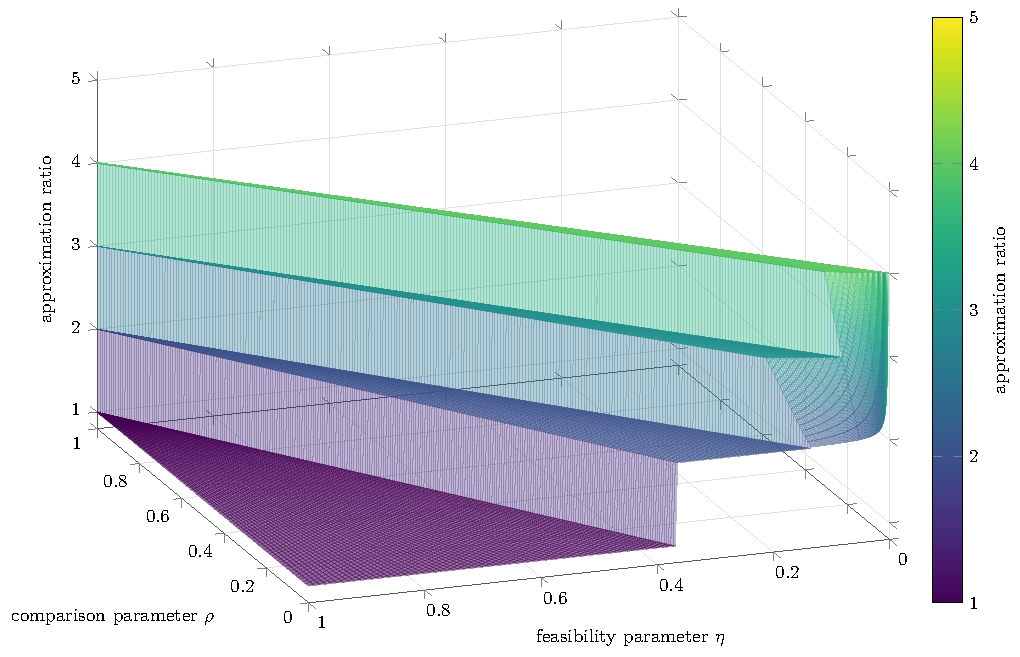
\includegraphics[width=0.94\textwidth]{figures/generated/tree_approximation_ratio_3d_plot.pdf}
  \caption{Combined tree approximation guarantee $\Gamma_{\mathrm{tree}}(\rho,\eta)$ from Corollary~\ref{cor:tree-best-bicriteria}, over $0<\rho<\eta<1$ (shown for $0.005\leq\rho\leq0.995$). Below the threshold, the height is the minimum of the anchored-LP, recursive, and hybrid bounds; above it, the direct dynamic program gives ratio $1$. Heights are capped at $12$. The plateaus reflect floor-log terms in the recursive and hybrid bounds.}
  \label{fig:tree-approximation-ratio-3d}
\end{figure}
